
\begin{infocard}{Volumen de un prisma recto}
    El volumen de un prisma recto de altura $h$, y cuyo polígono base tiene un área $A_B$, se obtiene mediante la expresión:
    \[
        V = A_B h
    \]
    \begin{figure}[H]
        \centering
        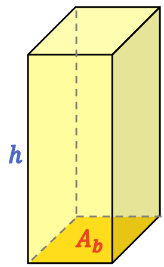
\includegraphics[width=0.45\textwidth]{../images/20230319192423}
        \caption{}
        \label{fig:20230319192423}
    \end{figure}
    
    Si el polígono base es un polígono regular (todos sus lados iguales), entonces:
    \[
        V = A_B h = \dfrac{\left( P \times a \right)}{2} (h) = \dfrac{n \times l \times a \times h}{2}
    \]
    donde $A_B$ es el área del polígono regular de la base, $P$ es el perímetro; $a$, la apotema; $n$, el número de
    lados; $l$, la medida del lado y $h$, la altura.
\end{infocard}



